\section{Date: 2026-09-27}
\noindent \textbf{Series ID: CIU1010000500000I} 

\noindent This series is titled Employment Cost Index: Total compensation for All Civilian workers in Production, transportation, and material moving and has a frequency of Quarterly. The units are Index Dec 2005=100 and the seasonal adjustment is Not Seasonally Adjusted.The observation start date is 2001-01-01 and the observation end date is 2026-04-01.The popularity of this series is 1. \\ 

\noindent \textbf{Series ID: USINTDCSJPY} 

\noindent This series is titled U.S. Intervention: With-Customer Transactions in the JPY/USD (Millions of USD) and has a frequency of Daily, 7-Day. The units are Millions of USD and the seasonal adjustment is Not Seasonally Adjusted.The observation start date is 1973-03-02 and the observation end date is 2011-05-31.The popularity of this series is 4. \\ 

\subsection{Raw Regression}
\noindent Regresses the two series against each other directly. A significant result here can come just as easily from both series sharing a long-run trend as from any real relationship.

\begin{center}
\begin{tabular}{lclc}
\toprule
\textbf{Dep. Variable:}                 & value\_fred\_USINTDCSJPY & \textbf{  R-squared:         } &       nan   \\
\textbf{Model:}                         &           OLS            & \textbf{  Adj. R-squared:    } &       nan   \\
\textbf{Method:}                        &      Least Squares       & \textbf{  F-statistic:       } &       nan   \\
\textbf{Date:}                          &     Sun, 27 Sep 2026     & \textbf{  Prob (F-statistic):} &      nan    \\
\textbf{Time:}                          &         15:52:42         & \textbf{  Log-Likelihood:    } &       inf   \\
\textbf{No. Observations:}              &              31          & \textbf{  AIC:               } &      -inf   \\
\textbf{Df Residuals:}                  &              29          & \textbf{  BIC:               } &      -inf   \\
\textbf{Df Model:}                      &               1          & \textbf{                     } &             \\
\textbf{Covariance Type:}               &        nonrobust         & \textbf{                     } &             \\
\bottomrule
\end{tabular}
\begin{tabular}{lcccccc}
                                        & \textbf{coef} & \textbf{std err} & \textbf{t} & \textbf{P$> |$t$|$} & \textbf{[0.025} & \textbf{0.975]}  \\
\midrule
\textbf{const}                          &            0  &            0     &       nan  &           nan        &            0    &            0     \\
\textbf{value\_fred\_CIU1010000500000I} &            0  &            0     &       nan  &           nan        &            0    &            0     \\
\bottomrule
\end{tabular}
\begin{tabular}{lclc}
\textbf{Omnibus:}       &    nan & \textbf{  Durbin-Watson:     } &      nan  \\
\textbf{Prob(Omnibus):} &    nan & \textbf{  Jarque-Bera (JB):  } &      nan  \\
\textbf{Skew:}          &    nan & \textbf{  Prob(JB):          } &      nan  \\
\textbf{Kurtosis:}      &    nan & \textbf{  Cond. No.          } & 1.18e+03  \\
\bottomrule
\end{tabular}
%\caption{OLS Regression Results}
\end{center}

Notes: \newline
 [1] Standard Errors assume that the covariance matrix of the errors is correctly specified. \newline
 [2] The condition number is large, 1.18e+03. This might indicate that there are \newline
 strong multicollinearity or other numerical problems.

\begin{figure}
\centering
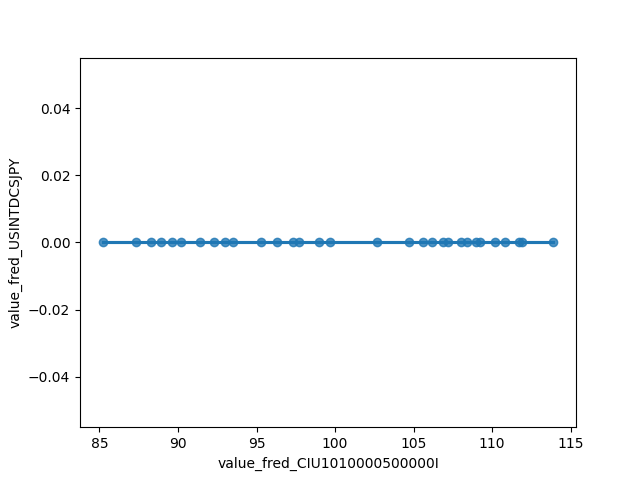
\includegraphics[scale = 0.9]{plots/plot_2026-09-27.png}
\caption{Raw Regression Plot for 2026-09-27}
\end{figure}
\newpage
\subsection{Detrended Regression}
\noindent Regresses the residuals of each series after removing its own linear time trend, so a shared trend can no longer drive the result on its own. A relationship that stays significant here is better evidence of a genuine link between the two series.

\begin{center}
\begin{tabular}{lclc}
\toprule
\textbf{Dep. Variable:}                            & value\_fred\_USINTDCSJPY\_detrended & \textbf{  R-squared:         } &       nan   \\
\textbf{Model:}                                    &                 OLS                 & \textbf{  Adj. R-squared:    } &       nan   \\
\textbf{Method:}                                   &            Least Squares            & \textbf{  F-statistic:       } &       nan   \\
\textbf{Date:}                                     &           Sun, 27 Sep 2026          & \textbf{  Prob (F-statistic):} &      nan    \\
\textbf{Time:}                                     &               15:52:43              & \textbf{  Log-Likelihood:    } &       inf   \\
\textbf{No. Observations:}                         &                    31               & \textbf{  AIC:               } &      -inf   \\
\textbf{Df Residuals:}                             &                    29               & \textbf{  BIC:               } &      -inf   \\
\textbf{Df Model:}                                 &                     1               & \textbf{                     } &             \\
\textbf{Covariance Type:}                          &              nonrobust              & \textbf{                     } &             \\
\bottomrule
\end{tabular}
\begin{tabular}{lcccccc}
                                                   & \textbf{coef} & \textbf{std err} & \textbf{t} & \textbf{P$> |$t$|$} & \textbf{[0.025} & \textbf{0.975]}  \\
\midrule
\textbf{const}                                     &            0  &            0     &       nan  &           nan        &            0    &            0     \\
\textbf{value\_fred\_CIU1010000500000I\_detrended} &            0  &            0     &       nan  &           nan        &            0    &            0     \\
\bottomrule
\end{tabular}
\begin{tabular}{lclc}
\textbf{Omnibus:}       &    nan & \textbf{  Durbin-Watson:     } &      nan  \\
\textbf{Prob(Omnibus):} &    nan & \textbf{  Jarque-Bera (JB):  } &      nan  \\
\textbf{Skew:}          &    nan & \textbf{  Prob(JB):          } &      nan  \\
\textbf{Kurtosis:}      &    nan & \textbf{  Cond. No.          } &     1.38  \\
\bottomrule
\end{tabular}
%\caption{OLS Regression Results}
\end{center}

Notes: \newline
 [1] Standard Errors assume that the covariance matrix of the errors is correctly specified.

\begin{figure}
\centering
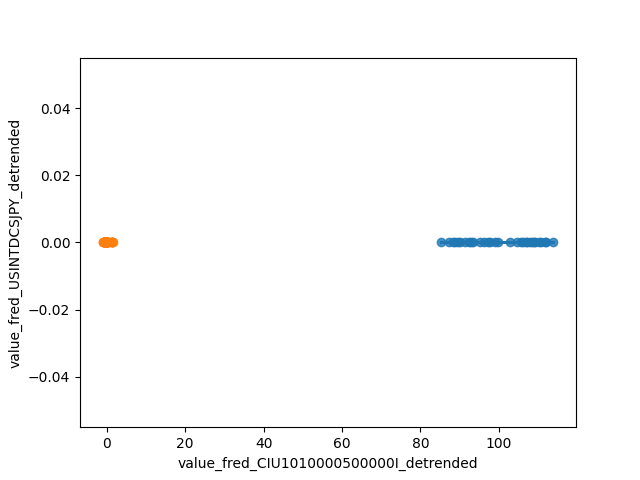
\includegraphics[scale = 0.9]{plots/plot_2026-09-27_detrended.png}
\caption{Detrended Regression Plot for 2026-09-27}
\end{figure}
\newpage
